\chapter{Approach}\label{sec:approach}

Two kind of approaches will be proposed. One one side, local approaches based on the PTAM implementation, where two steps are performed. The first step has been named \textit{Place Recognition} and the second \textit{Real Pose Recognition}. Multiple methods will be proposed to solve the second step. Then, on the other side, a global approach will be proposed. In this case machine learning methods (\textit{ferns}) will be used to recognize points in space.

\section{PTAM method}
\label{sec:ptam_method}

PTAM is a VO algorithm based on keyframes and so the relocalization method proposed is based on keyframes as well. Every keyframe has asociated with it a camera pose that will be used to relocalize. During the relocalization there are two steps involved. We have called the first step \textit{Place Recognition} and the second \textit{Real Pose Finder}.

\subsection{Place Recognition}
\label{ssub:place_recognition}

During this step, the algorithm tries to find the keyframe image most similar to the last acquired image. The pose associated with the most similar keyframe is used as an initial rough estimation of the current pose. The similarity score should be resistant to view point because the new acquired image will, most probably, never be taken from the same pose as any of the keyframes. Also it should be fast to compute.\\

The used similarity score is the Cross Correlation between images meaning the sum of the squared error between two zero-mean images. To make to computation faster both images are resized become $40\times30$. Then, to make the images more resistant to view point changes it is blurred with a $3\times3$ Gaussian kernel with $\sigma=2.5$. The resulting storied image is a resized, blurred and zero-mean image called \textit{small-blurry-image}.\\

During the normal map building pipeline this image is computed and stored every time a new keyframe is added to the map. And then, during the relocalization, the sum of squared difference between every stored \textit{small-blurry-image} and the last acquired frame is computed to find the most similar keyframe and then use its pose as an initial estimation of the current camera pose.\\

\subsubsection{Method validation}
\label{ssub:cc_method_validation}

To evaluate the method the real distance between two frames is going to be compared with the Cross Correlation value described above. Far away frames should be dissimilar and close by frames should be more similar and have a lower CC value. In figure \ref{fig:real_distance_confusion_matrix} can be seen the pair distances between image using the real pose while in figure \ref{fig:CC_confusion_matrix} there is the approximated pair distances using the CC value as distance. It can be seen that they have a similar distribution. Also the correlation of 0.4337 shows that one explains the other in most cases.\\

\begin{figure}
  \begin{subfigure}[b]{0.60\linewidth}
          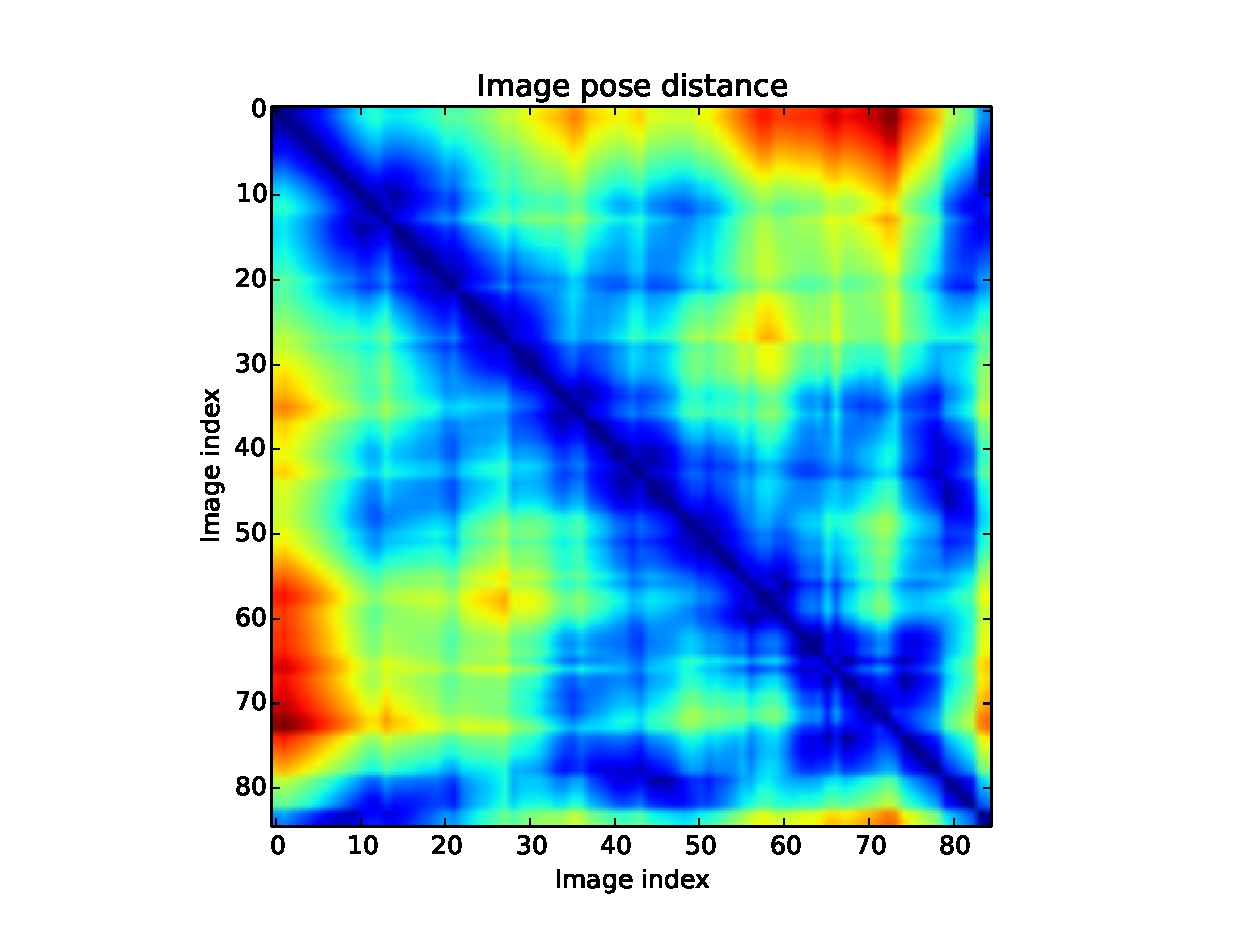
\includegraphics[width=\linewidth]{img/demo_1_1_CC_real_similarity_matrix.eps}
          \caption{Image to image real distance between the keyframe pose}                
          \label{fig:real_distance_confusion_matrix}
  \end{subfigure}   
  \qquad
  \begin{subfigure}[b]{0.60\linewidth}
         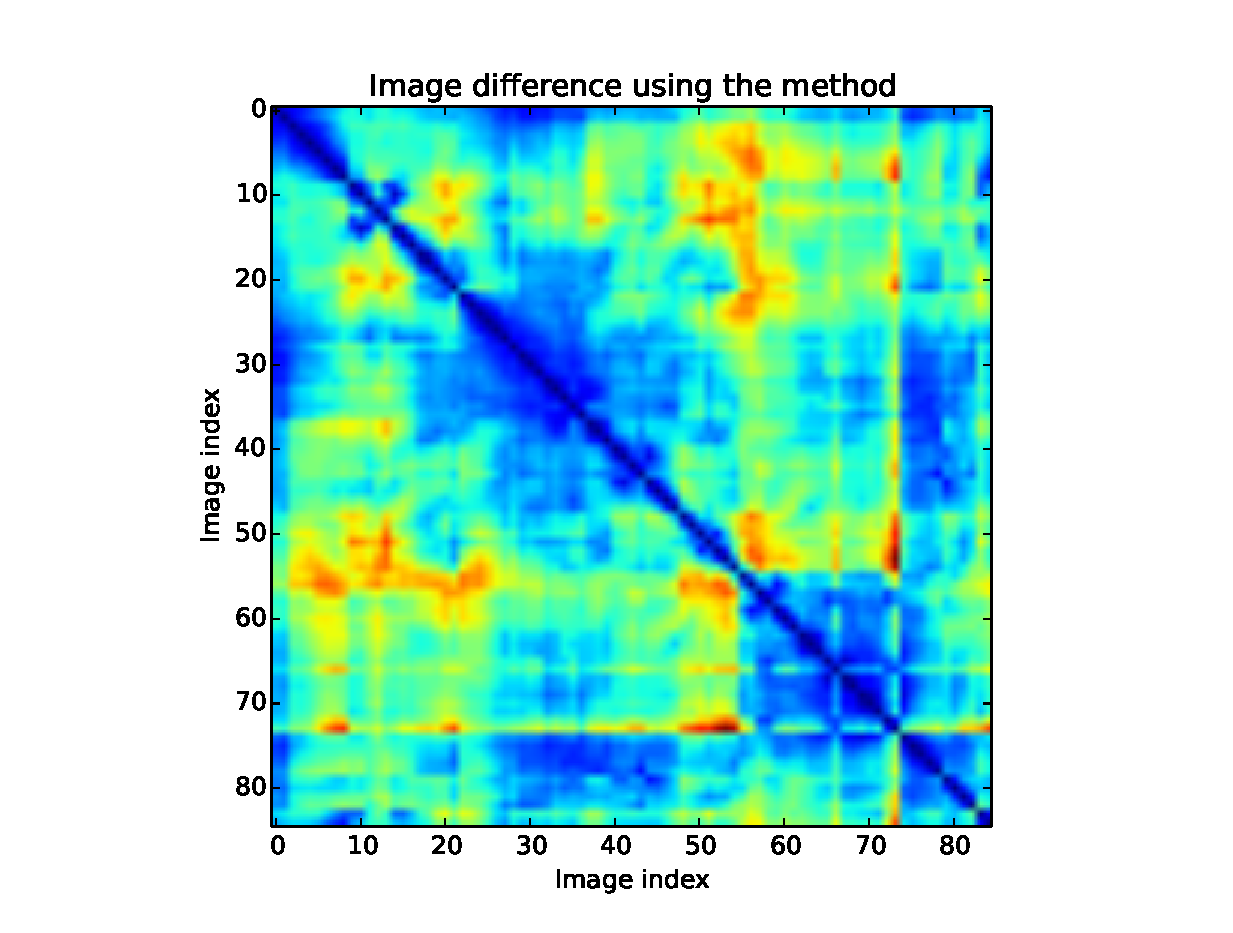
\includegraphics[width=\linewidth]{img/demo_1_1_CC_CC_similarity_matrix.eps}
         \caption{Image to image distance approximated using the Cross Correlation value}                
         \label{fig:CC_confusion_matrix}
  \end{subfigure}
  \caption{}
\end{figure}


Finally, to show that this method can be used, for every image the most CC similar image was taken being it real $K$ closest image. Ideally the most CC similar image should always be the closest image. In figure \ref{fig:K_closest} there is the count of occurrences of each $K$. It can be seen that most images resolve to the first or second closest image using this method.\\

\begin{figure}[!htbp]
  \centering
  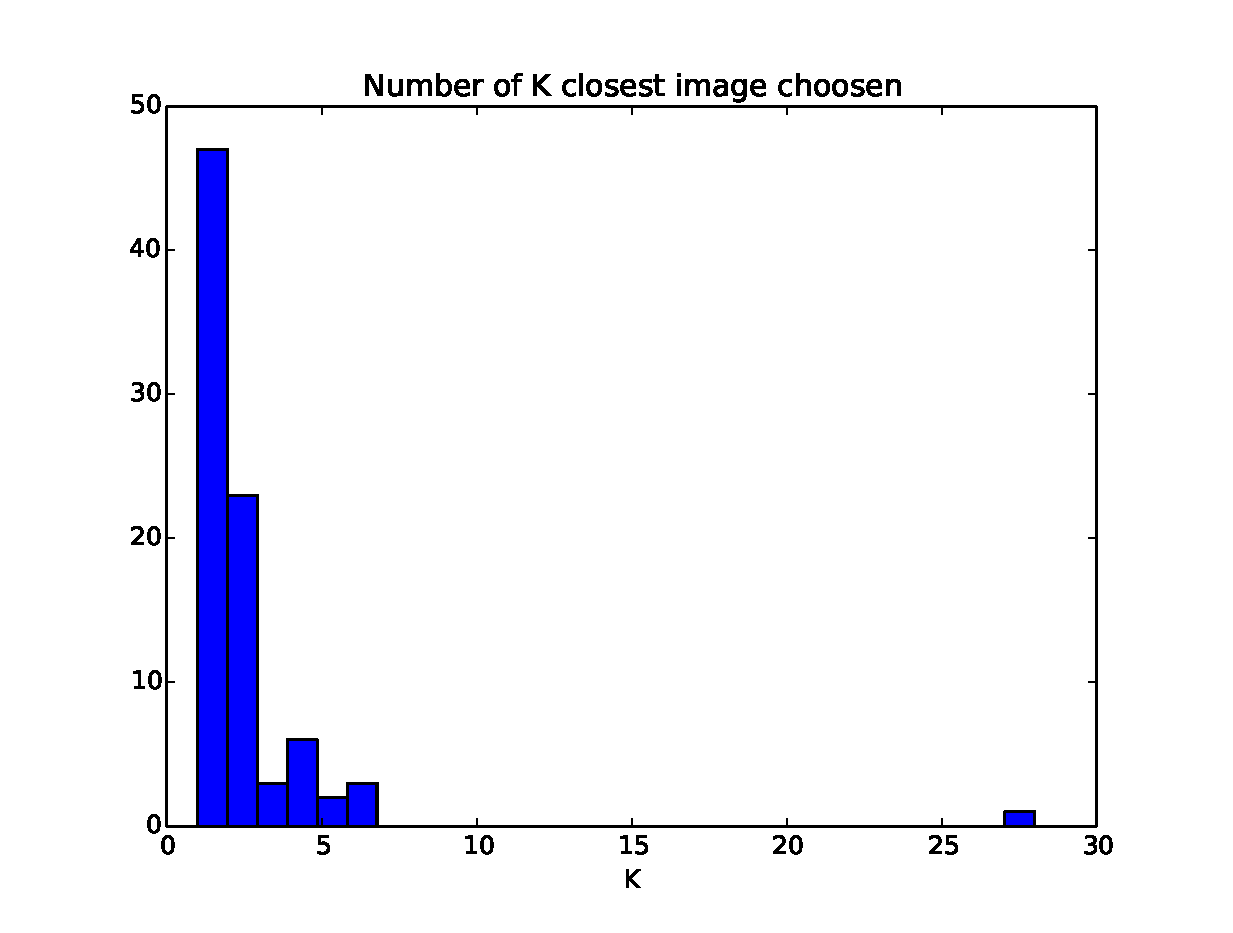
\includegraphics[width=9cm]{img/demo_1_1_CC_choose_distribution.eps}
  \caption{Distribution of closest chosen images using CC}
  \label{fig:K_closest}
\end{figure}


\begin{figure}[!htpb]
  \centering
  \begin{subfigure}[b]{0.6\linewidth}
    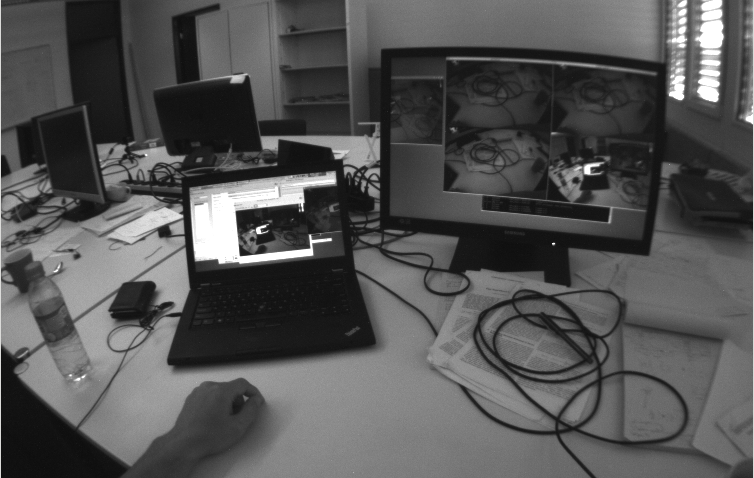
\includegraphics[width=\linewidth]{img/query_1.png}
    \caption{Query image}
    \label{fig:query_1}
  \end{subfigure}
  \quad
  \begin{subfigure}[b]{0.6\linewidth}
    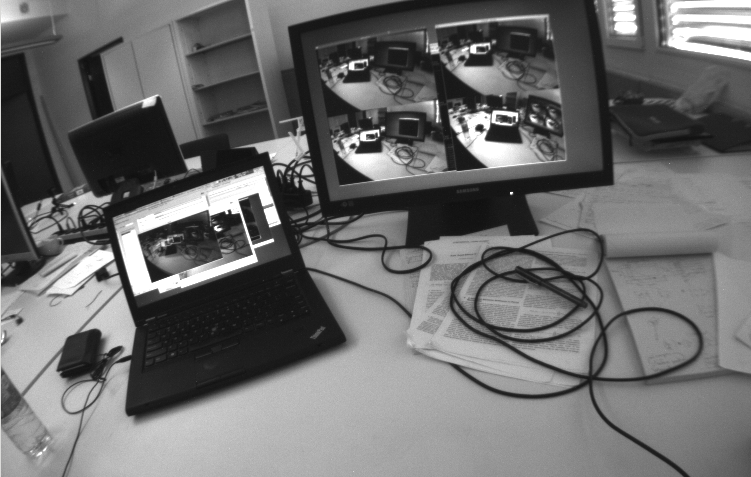
\includegraphics[width=\linewidth]{img/best_match_1.png}
    \caption{Found closest image}
    \label{fig:best_match_1}
  \end{subfigure}
  \caption{}
  \label{fig:cc_example}
\end{figure}


In figure \ref{fig:cc_example} of what would the algorithm return for a given query image for which there is no pose information available. Figure \ref{fig:query_1} is the image seen by the camera at the moment of the relocalization and \ref{fig:best_match_1} is what the system found to be the most similar, closest, image using the CC procedure explained previously. In this case the to image's camera pose are not the same, but they should be similar enough in order to find the difference in posterior steps.\\

\subsection{Real Pose Finder}
\label{sub:real_pose_finder}

The second step of the relocalization algorithm from PTAM tries to refine the pose of the found to be most similar keyframe to explain the current pose of the camera. During this step, in the implementation from PTAM, only rotations are corrected. An image alignment through optimization algorithm (ESM)~\ref{sec:lucas_kanard} is used to find the $SE(2)$ transformation between the two and then an other minimization is performed to find a transformation in the world frame.\\

\subsubsection{Image alignment}
\label{ssub:image_alignment}




\subsubsection{World frame interpretation}
\label{ssub:world_frame_interpretation}

This transformation is not easily interpreted in $SE(3)$, a translation in pixels can mean different things in the world frame depending on the distance to the object. Also, in $SE(3)$ there are three angular DoF, not one. The found transformation can be interpreted in multiple ways in the world frame. In the PTAM implementation it is assumed that the translation will only involve rotations, and so, the next step is the mapping from $SE(2)$ to $SO(3)$.\\

A Gauss-Newton minimization algorithm is used to find the $SO(3)$ model that modifies the image in the same way as the found $SE(2)$ model. The minimization is over the $SO(3)$ parameters $\xi$ and the error is expressed as in~\ref{equ:so3_error}

\begin{equation}
  \delta_i(\xi) = T_{SE(2)}u_i - \pi(T_{SO(3)}(\xi) p_i) \qquad \text{where} \quad u_i = \pi(p_i)
  \label{equ:so3_error}
\end{equation}


where $u_i$ is a pixel position (during the implementation $u_0=(5,0)$ and $u_1=(-5,0)$ are used). Also the Jacobian of $\delta$ is needed during the minimization process.

\begin{equation}
  \frac{\partial \delta(\xi)}{\partial \xi} = -\frac{\partial \pi (b)}{\partial b}|_{b=p} \frac{\partial T_{SO(3)}(\xi)}{\partial\xi}|_{\xi=0} \quad p
\end{equation}

with

\begin{equation}
  \frac{\partial \pi(b)}{\partial b} |_{b=p} = \frac{f}{z}
  \begin{bmatrix}
    1 & 0 & -\frac{x}{z} \\
    0 & 1 & -\frac{y}{z}
  \end{bmatrix}
  \qquad \text{where} \quad 
  p = \begin{bmatrix} x \\ y \\ z \end{bmatrix} \quad \text{and} \quad f = \text{focal length}
\end{equation}

\begin{equation}
  \frac{\partial T_{SO(3)}(\xi)}{\partial \xi_k}  = G_k \qquad \text{where} \quad G = \text{$SO(3)$ Generator}
\end{equation}


\subsubsection{Method validation}
\label{ssub:esm_method_validation}

To visualize the results of the different optimization procedures described above, the found transformation has been applied to the image. In the first step, the $SE(2)$ transformation between two image is computed and the transformed image on every step is one of the used variables. In figure~\ref{fig:se2_transformation_1} can be seen the final transformation found from~\ref{fig:best_match_1} to~\ref{fig:query_1}. In figure~\ref{fig:se3_error_1} the error can be visualized, there it can be seen that translation and rotation are well corrected but there still is a misalignment caused mostly by a change on scale which is not taken into account during the alignment.\\

\begin{figure}[htpb]
  \centering
  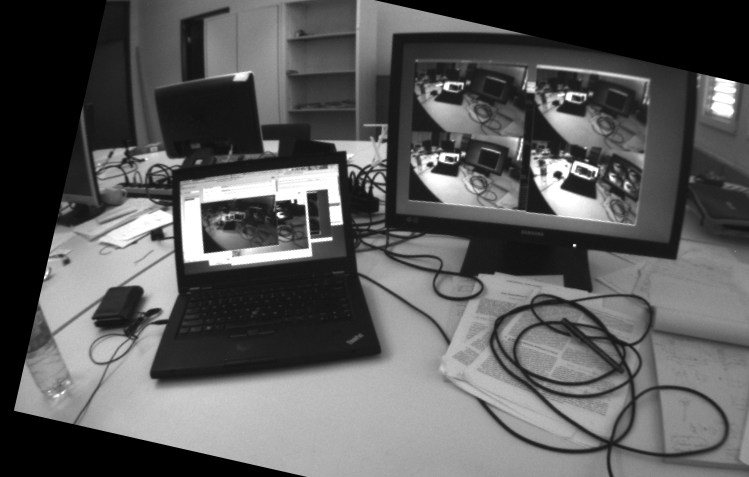
\includegraphics[width=0.6\linewidth]{img/se2_transformation_1.png}
  \caption{$SE(2)$ transformed image}
  \label{fig:se2_transformation_1}
\end{figure}

On the other side, during the second minimization where there $SO(3)$ translation is found, no image is actually involved, only two pixel coordinates. To generate a visualization of the translation the calibration of the camera is needed. Every pixel is unprotected form the image into the image plane, then the transformation is applied to it and finally it is projected back to the image. The result of the described procedure can be seen in figure~\ref{fig:so3_transformation_1}.\\

\begin{figure}[htpb]
  \centering
  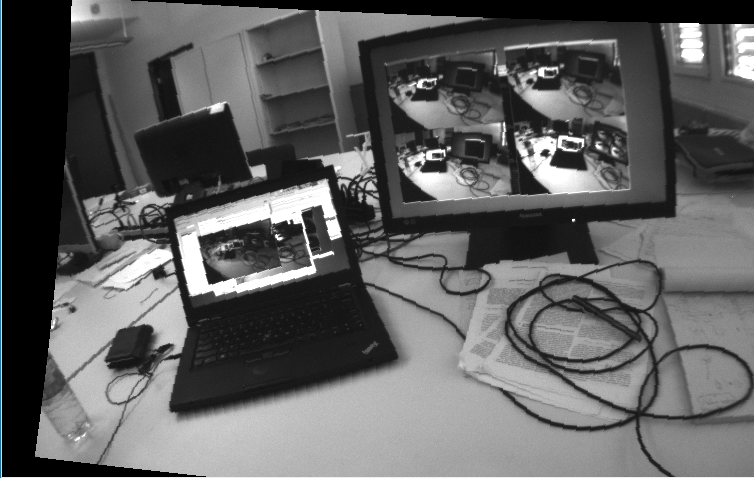
\includegraphics[width=0.6\linewidth]{img/so3_transformation_1.png}
  \caption{$SO(3)$ transformed image}
  \label{fig:so3_transformation_1}
\end{figure}

\begin{figure}[htpb]
  \centering
  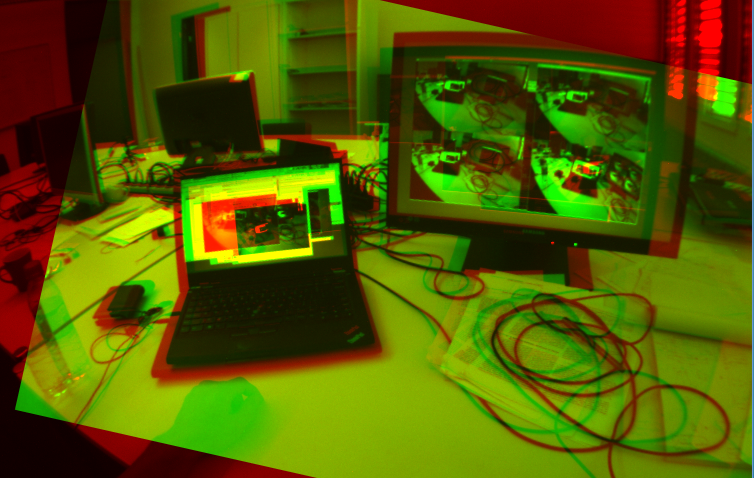
\includegraphics[width=0.6\linewidth]{img/se2_error_1.png}
  \caption{$SE(2)$ transformation error visualization}
  \label{fig:se3_error_1}
\end{figure}


\subsection{Real Pose Finder Alternative}
\label{sub:real_pose_finder_alternative}

During the mapping of an area the VO algorithm finds landmarks in the world frame which are associated with detected featured points in keyframes (i.e. every featured point in an image is related to a $3D$ position in the world frame). Given a new image, some extracted featured points can be related to a keyframe using the description-matching fashion which at the same time are related to world positions. From this information the full 6 DoF translation $SE(3)$ can be computed using the three point algorithm.\\

The 3pt algorithm and its implementation is described in \cite{kneipopengv}. In this case the described \textit{Central absolute pose} is dealt with.

\begin{figure}[htpb]
  \centering
  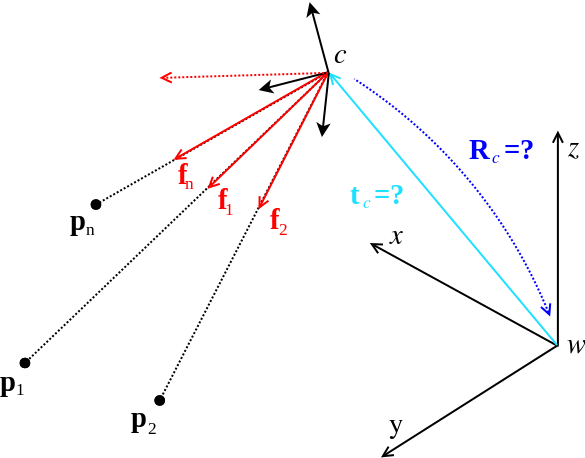
\includegraphics[width=0.6\linewidth]{img/absolute_central.png}
  \caption{From camera frame bearings (or image pixels if the camera calibration is available) and fix frame points the transformation between the two frames can be computed using the 3pt algorithm. Image from \cite{kneipopengv}}
  \label{fig:img/absolute_centra}
\end{figure}

First, descriptors from every featured point are extracted, both SIFT and SURF can be used updating a configuration file. Second, a brute force KNN matching is performed from all the extracted descriptors from on image and all the descriptors of the second image. The first, and second most similar descriptor are retrieved. Then, only good matches are kept, that is, using the matching technique described by Lowe, only matches with a descriptor ratio between the first and the second closest match of 0.8 or less are kept, only discriminant matches are used.\\

Finally, the 3pt algorithm is fed with the pixel positions from the query image and the landmarks from the other. Because there are still outliers after the described simple filtering, this process is run in RANSAC framework. \\


\subsubsection{Method validation}
\label{ssub:3pt_method_validation}

Figures~\ref{fig:3pt_matches} and~\ref{fig:3pt_inliers} are an example of the described above. The pose outputted was used to correctly relocalize and so it was correct.\\

The first part, where descriptors are extracted, matches and filtered, can be seen in figure~\ref{fig:3pt_matches}.  It can be seen that most matches are correct after this first filtering.\\

The inliers found during the RANSAC process can be seen in~\ref{fig:3pt_inliers}, it has to be kept in mind that the found transformation is not from image to image but from world, using world points, to frame. These world points can not be visualized and its precision could lead to not being included to the inliers group.\\

\begin{figure}[htpb]
  \centering
  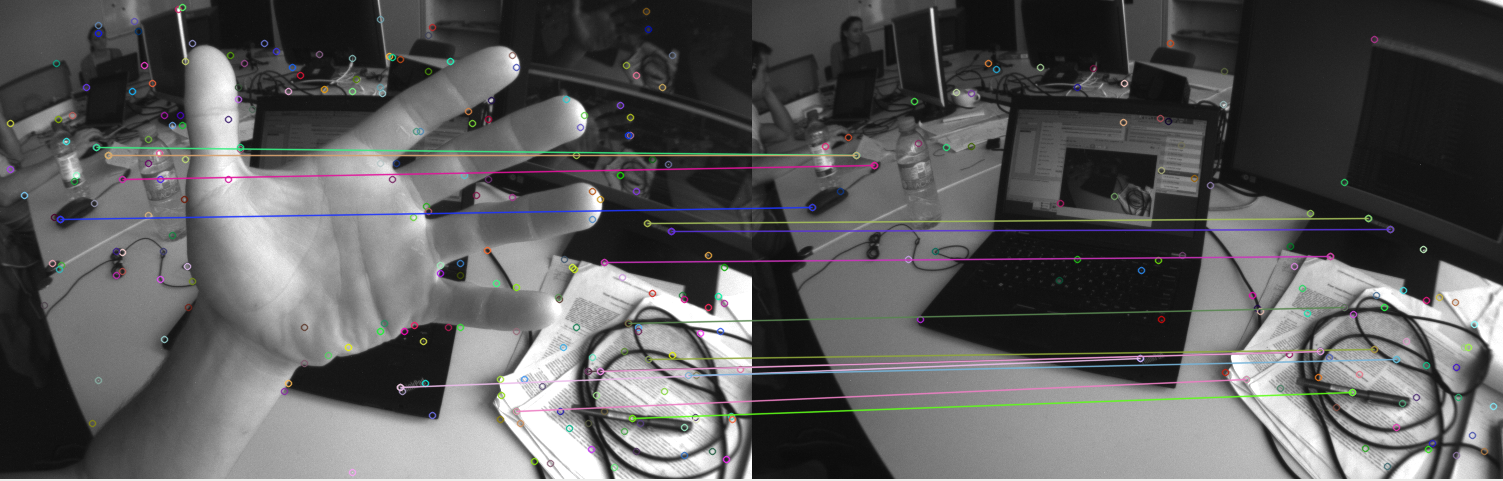
\includegraphics[width=1.0\linewidth]{img/3pt_matches_1.png}
  \caption{Accepted matches using SIFT}
  \label{fig:3pt_matches}
\end{figure}


\begin{figure}[htpb]
  \centering
  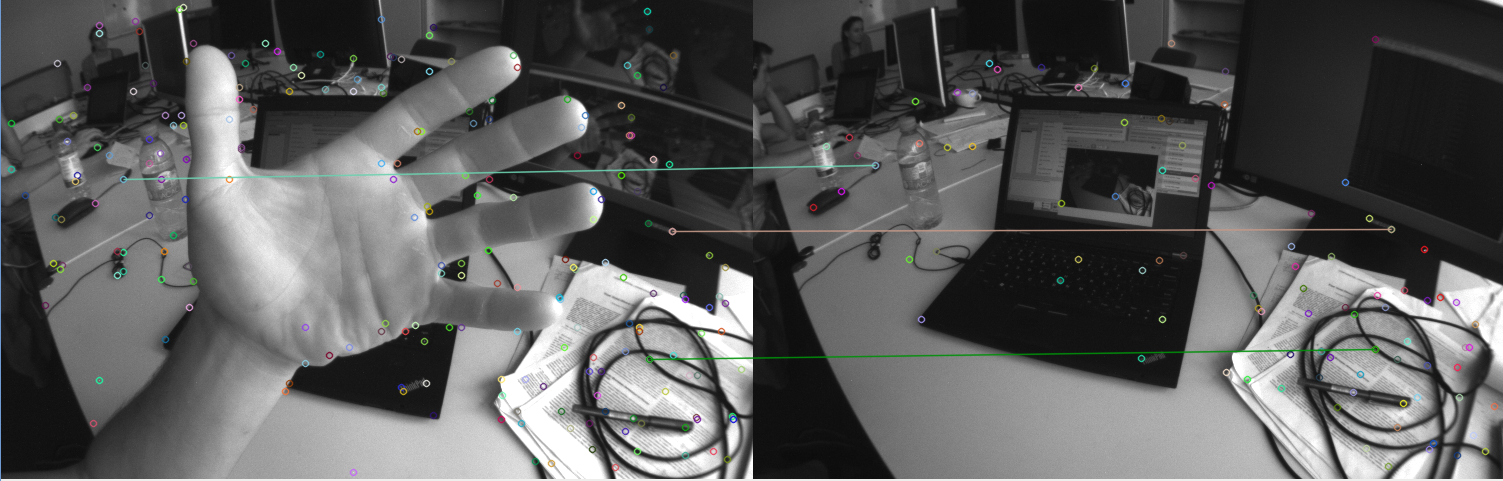
\includegraphics[width=1.0\linewidth]{img/3pt_inliers_1.png}
  \caption{Inliers from RANSAC used to calculate the pose with the three-point algorithm }
  \label{fig:3pt_inliers}
\end{figure}


\section{Using ferns}
\label{sec:using_ferns}

As said previously with the three-point algorithm it is possible to recover the 6 DoF of the camera pose from the relation from pixel coordinates and points in space. In this case machine learning techniques are used to model this relationship. In the classifier scheme, an object in space is a class and multiple views seen from the camera should all be classified as this class.\\

A \textit{fern} is a descriptor made from a set of binary tests~\ref{eq:fern_test}, made in a similarly  to random forests but flattened. When used as a classifier every possible evaluation of a \textit{fern} will contain a posterior provability distribution for every class, like random forests' final leafs do.\\

\begin{equation}
  f_j =
  \left\{
    \begin{array}{l l}
      1, & \text{if} \quad I(d_j,1) < I(d_j,2) \\
      0, & \text{otherwise}
    \end{array}
  \right
  \label{eq:fern_test}
\end{equation}

The result of the tests is encoded into the bits of an unsigned integer ~\ref{lst:fern_evaluation}. If a \textit{fern} has $S$ tests then its representation can have $K=2^{S}$ possible values which are then used  as index of its posterior distribution.\\

\lstset{language=C++,numbers=none,caption=Fern evaluation, label=lst:fern_evaluation}
\begin{lstlisting}[frame=lines]
uint8_t fern = 0;
for (size_t j = 0; j < S; ++j)
{
  //Shift bits
  fern <<= 1;
  if (I(d_j,1) < I(d_j,2))
  {
    //Change last bit
    fern++;
  }
}
\end{lstlisting}

One \testit{fern} is usually not descriptive enough to correctly classify, in \cite{Ozuysal2010} it is claimed that with 50 \testit{ferns} and $S=11$ a problem with 200 different classes is tractable. In memory, it would involve $50\times2^{11}\times200 = 20480000$ elements to be stored in memory. If these are stored as \textit{float} then 78 MB are needed, which is tractable. It should be noticed that the problem does not scale well on $S$, but at the same time, it is the most critic parameter.\\


\subsection{Seminaive Bayesian Approach}
\label{sub:seminaive_bayesian_approach}

Let $c_i, i = 1,\ldots,H$ be a set of classes and $f_j, j=1,\ldots,N$ be a set of binary tests~\ref{eq:fern_test} calculated over an image patch that is being classified. Formally, we are looking for

\begin{equation}
  \^c_i = \underset{c_i}{\text{argmax}} \quad P(C = c_i | f_1, f_2, \ldots, f_N)
\end{equation}

then, Bayes' formula tells

\begin{equation}
  P(C = c_i | f_1, f_2, \ldots, f_N) = \frac{P(f_1,f_2,\ldots,f_N \arrowvert C=c_i) P(C=c_i)}{P(f_1,f_2,\ldots,f_N)}
\end{equation}

Assuming a uniform prior and since the denominator is a scaling factor the problem is reduced to

\begin{equation}
  \^c_i = \underset{c_i}{\text{argmax}} \quad P(f_1, f_2, \ldots, f_N | C = c_i)
\end{equation}

Since this simple tests are very simple many of them are needed ($N \approx 300$), the storage of joint probabilities for every outcome is no feasible because $2^N$ entries for each class would be needed. One way to avoid this storage is to assume total independence between tests, this way the class provability distributions could be calculated like

\begin{equation}
  P(f_1, f_2, \ldots, f_N | C = c_i) = \prod^{N}_{j=1}P(f_j | C = c_i)
\end{equation}

but this ignores the possible correlation between tests. With \testit{ferns} a trade off is achieved, tests are grouped in sets $F$ and then the conditional provability becomes

\begin{equation}
  P(f_1, f_2, \ldots, f_N | C = c_i) = \prod^{M}_{k=1} P(F_k | C = c_i)
\end{equation}

It can be seen here why $S$ is important, an increment in the number of tests in a \textit{fern} means an increment in the modelled correlation.\\

\subsection{Training}
\label{sub:training}

During the training step many different views of a world point are needed to correctly model it. In the original work \cite{Ozuysal2010} only one image is used to train and to generate more possible views of the objects multiple (about 10,000) randomly generated warps are applied to it, all this warped images are used for training. Those warps include affine transformations, noise addition and smoothing with a Gaussian kernel (with all the parameters randomly picked from a uniform distribution).\\

In the studied case here, the algorithm can already provide multiple real views of the object (around 5-10), but still on each patch many randomly generated warps are applied and used to train (usually 100). In this case, the warps are simplified to include only image rotation and scale.\\

During the training, every warped patch is evaluated with every \textit{fern}. The count of a class evaluation on each \textit{fern} is performed along with the count of per class patches used. Those values are used during the classification step to calculate the provability distributions

\begin{equation}
  p_{k,c_i} = \frac{N_{k,c_i} + N_r}{N_{c_i} + K \times N_r}
\end{equation}

where $N_{k,c_i}$ is the number views of class $c_i$ that evaluates to $k$ and $N_{c_i}$ is the number of views of class $c_i$ to train. A regularization term $N_r = 1$ is used to avoid provabilities evaluating to zero.\\


\subsubsection{Method Validation}
\label{ssub:ferns_method_validation}

To validate the classifier a small test has been set up. One image is taken and from it 30 random patches are used to train the classifier. Then, 100 random warps are applied to those patches and classified. This process is reproduced 100 times. \\


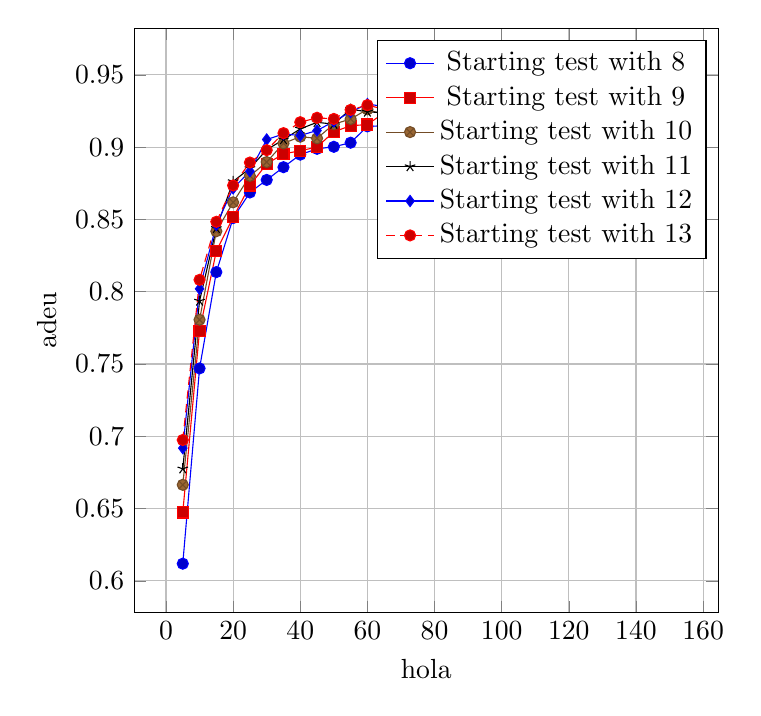
\begin{tikzpicture}
\begin{axis}[
height=9cm,
width=9cm,
grid=major,
xlabel=hola,
ylabel=adeu
]

\addplot coordinates
{
  (  5,0.611906)
  ( 10,0.746953)
  ( 15,0.81354 )
  ( 20,0.85091 )
  ( 25,0.868608)
  ( 30,0.877294)
  ( 35,0.8861  )
  ( 40,0.894782)
  ( 45,0.898805)
  ( 50,0.900189)
  ( 55,0.903035)
  ( 60,0.914335)
  ( 65,0.91471 )
  ( 70,0.909981)
  ( 75,0.917943)
  ( 80,0.91386 )
  ( 85,0.91913 )
  ( 90,0.91375 )
  ( 95,0.918169)
  (100,0.922886)
  (105,0.918348)
  (110,0.922474)
  (115,0.923372)
  (120,0.918301)
  (125,0.921832)
  (130,0.92336 )
  (135,0.926459)
  (140,0.929506)
  (145,0.925352)
  (150,0.927638)
};
\addlegendentry{Starting test with 8}

\addplot coordinates
{
  (  5,0.647313)
  ( 10,0.773075)
  ( 15,0.828111)
  ( 20,0.851374)
  ( 25,0.873437)
  ( 30,0.8884  )
  ( 35,0.895329)
  ( 40,0.897437)
  ( 45,0.900028)
  ( 50,0.9106  )
  ( 55,0.914759)
  ( 60,0.915583)
  ( 65,0.923693)
  ( 70,0.920662)
  ( 75,0.922914)
  ( 80,0.924085)
  ( 85,0.919677)
  ( 90,0.922637)
  ( 95,0.929174)
  (100,0.926049)
  (105,0.920981)
  (110,0.927521)
  (115,0.927604)
  (120,0.928871)
  (125,0.933295)
  (130,0.932722)
  (135,0.931251)
  (140,0.934049)
  (145,0.932926)
  (150,0.932927)
};
\addlegendentry{Starting test with 9}

\addplot coordinates
{
  (  5,0.666433)
  ( 10,0.780569)
  ( 15,0.841805)
  ( 20,0.861785)
  ( 25,0.880106)
  ( 30,0.889655)
  ( 35,0.902569)
  ( 40,0.907179)
  ( 45,0.90605 )
  ( 50,0.915868)
  ( 55,0.919375)
  ( 60,0.926114)
  ( 65,0.922165)
  ( 70,0.928139)
  ( 75,0.927301)
  ( 80,0.928778)
  ( 85,0.937536)
  ( 90,0.927311)
  ( 95,0.932855)
  (100,0.930164)
  (105,0.937211)
  (110,0.934534)
  (115,0.931139)
  (120,0.933956)
  (125,0.934776)
  (130,0.936754)
  (135,0.939867)
  (140,0.937029)
  (145,0.933167)
  (150,0.931782)
};
\addlegendentry{Starting test with 10}

\addplot coordinates
{
  (  5,0.677536)
  ( 10,0.793594)
  ( 15,0.843825)
  ( 20,0.876226)
  ( 25,0.88533 )
  ( 30,0.898161)
  ( 35,0.905165)
  ( 40,0.912597)
  ( 45,0.917115)
  ( 50,0.915842)
  ( 55,0.926304)
  ( 60,0.924285)
  ( 65,0.923873)
  ( 70,0.926913)
  ( 75,0.930721)
  ( 80,0.932727)
  ( 85,0.930798)
  ( 90,0.932624)
  ( 95,0.932255)
  (100,0.93505 )
  (105,0.940008)
  (110,0.93772 )
  (115,0.941688)
  (120,0.937759)
  (125,0.94243 )
  (130,0.936116)
  (135,0.944297)
  (140,0.9423  )
  (145,0.942671)
  (150,0.943069)
};
\addlegendentry{Starting test with 11}

\addplot coordinates
{
  (  5,0.691823)
  ( 10,0.801977)
  ( 15,0.84622 )
  ( 20,0.871452)
  ( 25,0.88331 )
  ( 30,0.905238)
  ( 35,0.909072)
  ( 40,0.908045)
  ( 45,0.911443)
  ( 50,0.917715)
  ( 55,0.924286)
  ( 60,0.929765)
  ( 65,0.928045)
  ( 70,0.931749)
  ( 75,0.926873)
  ( 80,0.934515)
  ( 85,0.932165)
  ( 90,0.944389)
  ( 95,0.937691)
  (100,0.933969)
  (105,0.942654)
  (110,0.941569)
  (115,0.943457)
  (120,0.939013)
  (125,0.943969)
  (130,0.941761)
  (135,0.945584)
  (140,0.940012)
  (145,0.943518)
  (150,0.942326)
};
\addlegendentry{Starting test with 12}

\addplot coordinates
{
  (  5,0.697447) 
  ( 10,0.80819 )
  ( 15,0.848335)
  ( 20,0.873454)
  ( 25,0.889331)
  ( 30,0.897887)
  ( 35,0.909651)
  ( 40,0.917206)
  ( 45,0.920271)
  ( 50,0.919475)
  ( 55,0.925751)
  ( 60,0.929024)
  ( 65,0.926151)
  ( 70,0.929887)
  ( 75,0.932009)
  ( 80,0.93693 )
  ( 85,0.937005)
  ( 90,0.940786)
  ( 95,0.9351  )
  (100,0.938899)
  (105,0.941297)
  (110,0.943029)
  (115,0.942325)
  (120,0.942684)
  (125,0.946154)
  (130,0.9396  )
  (135,0.948533)
  (140,0.948097)
  (145,0.944212)
  (150,0.944371)
};
\addlegendentry{Starting test with 13}

\end{axis}
\end{tikzpicture}


hola
































































\chapter{To be removed}
\label{cha:chapter_name}



Describe the main steps in your algorithm. An illustration is always helpful.\\

Here are some \LaTeX~tips:


\section{Headings}

  Your report can be structured using several different types of headings. Use the commands \textbackslash\texttt{chapter}\{.\}, \textbackslash\texttt{section}\{.\}, \textbackslash\texttt{subsection}\{.\}, and \textbackslash\texttt{subsubsection}\{.\}. Use the asterisk symbol \texttt{*} to suppress numbering of a certain heading if necessary, for example, \textbackslash\texttt{section*}\{.\}.


\section{References}\label{sec:references}

  References to literature are included using the command \textbackslash\texttt{cite}\{.\}. For example \cite{KleinMurray2007,Strasdat2010WhyFilter}. Your references must be entered in the file \texttt{bibliography.bib}. Making changes or adding new references in the bibliography file can be done manually or by using specialized software such as \textit{JabRef} which is free of charge.

  Cross-referencing within the text is easily done using \textbackslash\texttt{label}\{.\} and \textbackslash\texttt{ref}\{.\}. For example, this paragraph is part of chapter~\ref{sec:approach}; more specifically on page~\pageref{sec:references}.

\section{Writing Equations}\label{sec:math}

  The most common way to include equations is using the \texttt{equation} environment. Use \textbackslash\texttt{eqref}\{.\} to reference an equation, e.g. \eqref{eq:leastsquares}.
  \begin{equation}\label{eq:leastsquares}
      \begin{aligned}
        C(\mathbf{x}) &= \frac{1}{2} \ \sum_{i \in \mathcal I} \sum_{k \in \mathcal K_i} \mathbf{e}_{i,k}(\mathbf{x})^T \ \mathbf{W}_{i,k}  \ \mathbf{e}_{i,k}(\mathbf{x})  \\
        \hat{\mathbf{x}}^{LS} &= \text{argmin}_\mathbf{x} \ C(\mathbf{x}),
      \end{aligned}
  \end{equation}

  \begin{equation}\label{eq:se3}
    \mathtt{T}_i = \begin{bmatrix}\mathbf{R}_i & \mathbf{p}_i \\ 0 & 1\end{bmatrix} \qquad \text{with} \quad \mathbf{R}_i \in SO(3), \ \ \mathbf{p} \in \mathbb{R}^3.
  \end{equation}

\section{Including Graphics}\label{sec:epsgraph}
  The easiest way to include figures in your document is to use pdf figures if you use \texttt{pdflatex} to compile. Figure \ref{img:notation} was created with the use of the open source program \texttt{ipe}.

  \begin{figure}[h]
     \centering
     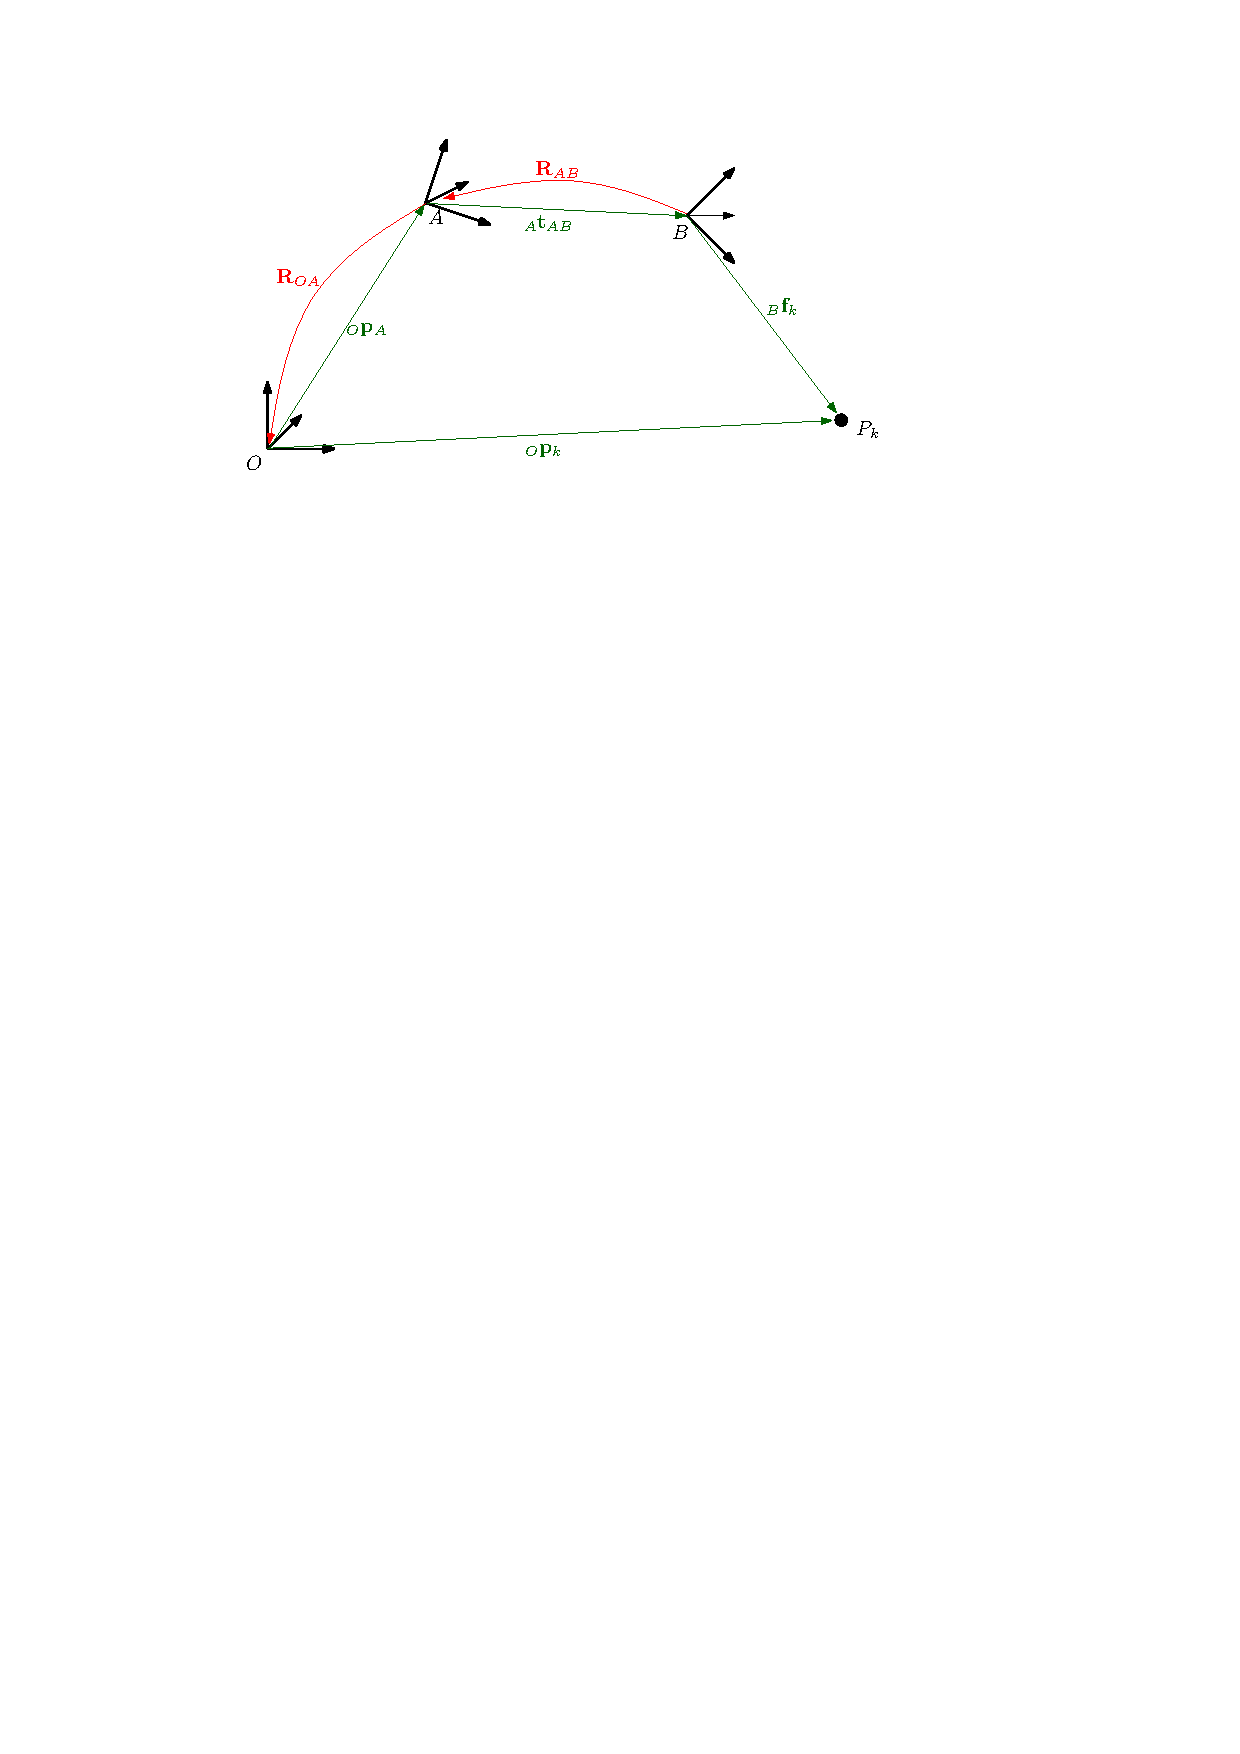
\includegraphics[width=0.6\textwidth]{img/notation.pdf}
     \caption{Example of a figure.}
     \label{img:notation}
  \end{figure}


\section{Including Code in your Document}

  You may include samples from your Matlab code using the \texttt{lstlistings} environment, for example
  \lstset{language=Matlab,numbers=none}
  \begin{lstlisting}[frame=lines, caption=Matlab Example, label=matlabexample]
  % Evaluate y = 2x
  for i = 1:length(x)

    y(i) = 2*x(i);

  end
  \end{lstlisting}

  \lstset{language=C++,numbers=none,caption=C++ Example, label=cppexample}
  \begin{lstlisting}[frame=lines]
  % sum all elements in a list
  int sum=0;
  for(list<int>::iterator it=mylist.begin(); it!=mylist.end(); ++it)
    sum += *it;
  \end{lstlisting}
